\part{Introduction}


\chapter{Overview}

Vue.js(读音 /vjuː/, 类似于 view) 是一套构建用户界面的 渐进式框架,Vue.js 的目标是通过尽可能简单的 API 实现响应的数据绑定和组合的视图组件。

在本地的HTML文件中通过如下方式来引入Vue就可以尝试Vue.js。

\begin{lstlisting}[language=HTML]
<html>
<head>
   <script src="path/to/vue.js"></script>
</head>
<body>
<div id="app">
   <p>{{ message }}</p>
</div>
</body>
<scritpt>
new Vue({
   el: '#app',
   data: {
      message: 'Hello Vue.js!'
   }
})
</script>
</html>
\end{lstlisting}

\begin{compactitem}
\item Vue的el指定一个视图模板;
\item Vue的实例创建一个VM对象。
\end{compactitem}

\section{Kernel}

vue.js具有简单小巧的核心和渐进式技术栈,足以应付任何规模的应用。

vue.js的运行文件使用gzip压缩后最小可以到17kb,其提供的超快虚拟 DOM可以实现最省心的优化。



\subsection{vue-kernel}

与其他重量级框架不同的是,Vue 采用自底向上增量开发的设计。Vue 的核心库只关注视图层,并且非常容易学习,非常容易与其它库或已有项目整合。

另一方面,Vue 完全有能力驱动采用单文件组件和 Vue 生态系统支持的库开发的复杂单页应用。

\subsection{vue-cli}


Vue.js 本身也提供配套工具(例如vue-cli)来开发单文件组件。


vue.js提供的一个命令行工具vue-cli可以用来搭建Vue项目的脚手架,用于快速搭建大型单页应用。

vue-cli提供了开箱即用的构建工具配置,带来现代化的前端开发流程。只需几分钟即可创建并启动一个带热重载、保存时静态检查以及可用于生产环境的构建配置的项目:


\begin{compactitem}
\item 全局安装vue-cli

\begin{lstlisting}[language=bash]
$ sudo npm install --global vue-cli
\end{lstlisting}

\item 创建一个基于 webpack 模板的新项目

\begin{lstlisting}[language=bash]
$ vue init webpack my-project
\end{lstlisting}

\item 安装依赖

\begin{lstlisting}[language=bash]
$ cd my-project
$ npm install
$ npm run dev
\end{lstlisting}
\end{compactitem}

注意,vue-cli要求用户事先了解Node.js和相关的构建工具(例如webpack),或者在熟悉Vue本身之后再使用vue-cli。





\section{Installation}


如果直接下载并用 <script> 标签引入vue.min.js,Vue 会被注册为一个全局变量。

\begin{lstlisting}[language=HTML]
<html>
<head>
   <script src="path/to/vue.js"></script>
</head>
<body>

</body>
</html>
\end{lstlisting}

在开发时使用vue.js的开发版本(非最小压缩版),遇到常见错误时,vue.js会给出友好的警告。

如果使用 Vue.js 构建大型应用,推荐使用 NPM 进行安装,而且NPM 能很好地和 Webpack 或 Browserify 等模块打包器配合使用。

\begin{compactitem}
\item 使用NPM全局安装vue.js的最新稳定版

\begin{lstlisting}[language=bash]
$ sudo npm install -g vue
\end{lstlisting}

\item 使用bower安装vue.js的最新稳定版本

\begin{lstlisting}[language=bash]
$ bower install vue
\end{lstlisting}
\end{compactitem}

独立下载版本或通过 Bower 安装的版本已用 UMD 包装,因此它们可以直接用作 AMD 模块。



如果需要使用Vue最新的功能和代码,用户可以自己在本地构建vue的开发版本。


\begin{lstlisting}[language=bash]
$ git clone https://github.com/vuejs/vue.git node_modules/vue
$ cd node_modules/vue
$ npm install
$ npm run build
\end{lstlisting}


\subsection{Standalone Build}


Vue.js有两种构建方式,独立构建和运行构建。它们的区别在于前者包含模板编译器而后者不包含,而且运行时构建比独立构建要轻量30\%,只有 17.14 Kb min+gzip大小。


模板(template)编译用于把 Vue 模板字符串编译成纯 JavaScript 渲染函数。如果想用 template 选项, 就需要编译。其中,模板编译器的职责是将模板字符串编译为纯 JavaScript 的渲染函数。如果想要在组件中使用 template 选项,那么就需要模板编译器。


\begin{compactitem}
\item 独立构建包含模板编译器并支持 template 选项。 它也依赖于浏览器的接口的存在,所以不能使用它来为服务器端渲染页面。
\item 运行时构建不包含模板编译器,因此不支持 template 选项,只能用 render 选项,但是即使使用运行时构建,在单文件组件中也依然可以写模板,因为单文件组件的模板会在构建时预编译为 render 函数。
\end{compactitem}






为了使用独立构建,可以在 webpack 配置中添加下面的别名:

\begin{lstlisting}[language=JavaScript]
resolve: {
    alias: {
        'vue$': 'vue/dist/vue.common.js'
    }
}
\end{lstlisting}

对于Browserify,可以添加一个别名到 package.json 中:

\begin{lstlisting}[language=JavaScript]
"browser": {
  "vue": "vue/dist/vue.common"
},
\end{lstlisting}



\subsection{Runtime-only Build}


默认 NPM 包导出的是 运行时 构建。

运行时构建(runtime+compiler)的优势在于文件体积小,但是不支持template选项。

Runtime-only: about 6KB lighter min+gzip, but templates (or any Vue-specific HTML) are ONLY allowed in .vue files - render functions are required elsewhere 


\section{Compatibility}


 Vue.js 支持所有兼容 ECMAScript 5 的浏览器。
 
 Vue.js 不支持 IE8 及其以下版本,因为 Vue.js 使用了 IE8 不能模拟的 ECMAScript 5 特性。
 
 \subsection{CSP}
 
 
 有些环境(例如 Google Chrome Apps)强制应用内容安全策略 (CSP) ,不能使用 new Function() 对表达式求值。
 
Vue.js提供了 CSP 兼容版本,注意Vue.js的独立构建取决于该功能编译模板,所以无法使用这些CSP环境。

另一方面,运行时构建的是完全兼容 CSP 的,因此当通过 Webpack + vue-loader 或者 Browserify + vueify 构建Vue.js时,在 CSP 环境中模板将被完美预编译到 render 函数中。


 


\section{Conditionals and Loops}

\subsection{v-if}



使用Vue.js可以控制切换一个元素的显示。


\begin{lstlisting}[language=HTML]
<div id="app-3">
  <p v-if="seen">Now you see me</p>
</div>
<script>
var app3=new Vue({
   el: '#app-3',
   data: {
       seen: true
   }
})
</script>
\end{lstlisting}

在控制台设置\texttt{app3.seen = false}会发现 “Now you see me” 消失了。


使用Vue.js不仅可以绑定 DOM 文本到数据,也可以绑定 DOM 结构到数据,同时Vue.js还提供了一个强大的过渡效果系统,可以在 Vue 插入/删除元素时自动应用过渡效果。

\subsection{v-for}

Vue.js也有一些其它指令,每个都有特殊的功能。例如, v-for 指令可以绑定数据到数组来渲染一个列表:

\begin{lstlisting}[language=HTML]
<div id="app-4">
  <ol>
    <li v-for="todo in todos">
      {{ todo.text }}
    </li>
  </ol>
</div>

<script>
var app4 = new Vue({
  el: '#app-4',
  data: {
    todos: [
      { text: 'Learn JavaScript' },
      { text: 'Learn Vue' },
      { text: 'Build something awesome' }
    ]
  }
})
</script>
\end{lstlisting}

在控制台里,输入\texttt{app4.todos.push(\{ text: 'New item' \})}会发现列表中多了一栏新内容。

\section{Handling User Input}


\subsection{v-on}


为了让用户和Vue应用进行互动,可以用 v-on 指令绑定一个监听事件用于调用 Vue 实例中定义的方法:

\begin{lstlisting}[language=HTML]
<div id="app-5">
  <p>{{ message }}</p>
  <button v-on:click="reverseMessage">Reverse Message</button>
</div>

<script>
var app5 = new Vue({
  el: '#app-5',
  data: {
    message: 'Hello Vue.js!'
  },
  methods: {
    reverseMessage: function () {
      this.message = this.message.split('').reverse().join('')
    }
  }
})
</script>
\end{lstlisting}

在这里的 reverseMessage 方法中,可以在没有接触 DOM 的情况下更新应用的状态,所有的 DOM 操作都由 Vue 来处理,代码只需要关注基本逻辑。


\subsection{v-model}


Vue 也提供了 v-model 指令,它使得在表单输入和应用状态中做双向数据绑定变得非常轻巧。




\begin{lstlisting}[language=HTML]
<div id="app-6">
  <p>{{ message }}</p>
  <input v-model="message">
</div>

<script>
var app6 = new Vue({
  el: '#app-6',
  data: {
    message: 'Hello Vue!'
  }
})
</script>
\end{lstlisting}


\section{Compose Components}


组件系统是Vue.js的重要概念,Vue.js的组件系统提供了一种抽象,从而可以用独立可复用的小组件来构建大型应用,这样几乎任意类型的应用的界面都可以通过组件系统来抽象为一个组件树。


\begin{figure}[htbp]
\centering
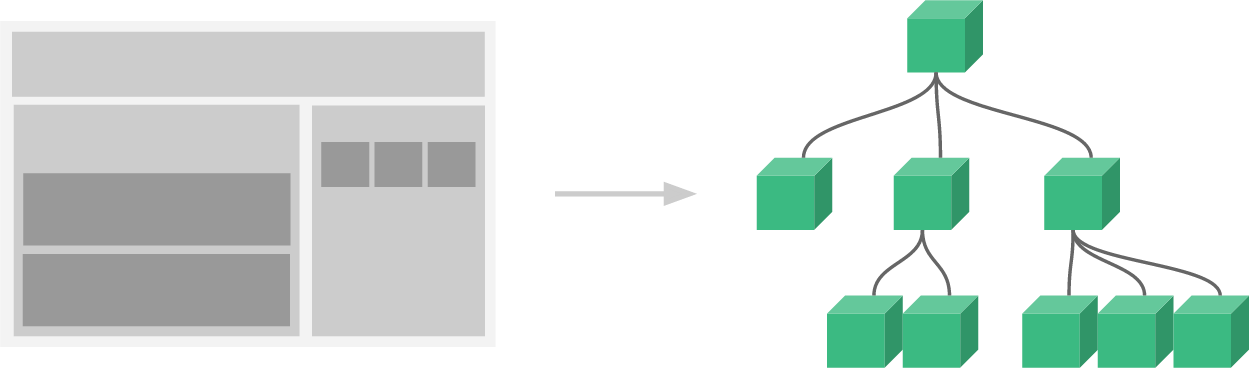
\includegraphics[scale=0.3]{components.png}
\caption{Vue.js组件系统}
\end{figure}

在一个大型应用中,为了使得开发过程可控,有必要将应用整体分割成一个个的组件。

\begin{lstlisting}[language=HTML]
<div id="app">
  <app-nav></app-nav>
  <app-view>
    <app-sidebar></app-sidebar>
    <app-content></app-content>
  </app-view>
</div>
\end{lstlisting}


Vue.js 组件非常类似于自定义元素——它是 Web 组件规范的一部分,而且实际上 Vue.js 的组件语法也参考了该规范。例如, Vue 组件实现了 Slot API 与 is 特性。

Vue.js组件和Web组件规范的关键的不同如下:

\begin{compactenum}
\item Web 组件规范仍然远未完成,并且没有浏览器实现。相比之下,Vue.js 组件不需要任何补丁,并且在所有支持的浏览器(IE9 及更高版本)之下表现一致。必要时,Vue.js 组件也可以放在原生自定义元素之内。
\item Vue.js 组件提供了原生自定义元素所不具备的一些重要功能,比如组件间的数据流,自定义事件系统,以及动态的、带特效的组件替换。
\end{compactenum}

在 Vue 里,一个组件实质上是一个拥有预定义选项的一个 Vue 实例:


\begin{lstlisting}[language=JavaScript]
// Define a new component called todo-item
Vue.component('todo-item', {
  template: '<li>This is a todo</li>'
})
\end{lstlisting}

在定义了一个组件之后就可以在另一个组件模板中写入它:

\begin{lstlisting}[language=HTML]
<ol>
  <!-- Create an instance of the todo-item component -->
  <todo-item></todo-item>
</ol>
\end{lstlisting}

最初,组件会为每个 todo 渲染同样的文本,实际上应该将数据从父作用域传到子组件,接下来可以修改组件的定义来让它能够接受一个 prop 字段:


\begin{lstlisting}[language=JavaScript]
Vue.component('todo-item',{
    // The todo-item component now accepts a
    // "prop", which is like a custom attribute.
    // This prop is called todo.
    props: ['todo'],
    template: '<li>{{ todo.text }}</li>
})
\end{lstlisting}

现在,可以使用 v-bind 指令将 todo 传到每一个重复的组件中:



\begin{lstlisting}[language=HTML]
<div id="app-7">
  <ol>
    <!-- Now we provide each todo-item with the todo object    -->
    <!-- it's representing, so that its content can be dynamic -->
    <todo-item v-for="item in groceryList" v-bind:todo="item"></todo-item>
  </ol>
</div>

Vue.component('todo-item', {
  props: ['todo'],
  template: '<li>{{ todo.text }}</li>'
})
var app7 = new Vue({
  el: '#app-7',
  data: {
    groceryList: [
      { text: 'Vegetables' },
      { text: 'Cheese' },
      { text: 'Whatever else humans are supposed to eat' }
    ]
  }
})
\end{lstlisting}


上述示例将应用分割成了两个更小的单元,子元素通过 props 接口实现了与父亲元素很好的解耦,现在可以在不影响到父应用的基础上,进一步为todo 组件改进更多复杂的模板和逻辑。

\chapter{Vue Prop}


在 Vue.js 中,父子组件的关系可以总结为 props down, events up,父组件通过 props 向下传递数据给子组件,子组件通过 events 给父组件发送消息。


\section{Prop}



组件实例的作用域是孤立的,这意味着不能并且不应该在子组件的模板内直接引用父组件的数据,Vue推荐使用 props 把数据传给子组件。


\begin{lstlisting}[language=JavaScript]
<div id="app">
    <child message="hello!"></child>
</div>
 
<script>
// 注册
Vue.component('child', {
  // 声明 props
  props: ['message'],
  // 同样也可以在 vm 实例中像 "this.message" 这样使用
  template: '<span>{{ message }}</span>'
})
// 创建根实例
new Vue({
  el: '#app'
})
</script>
\end{lstlisting}


prop的本质是父组件用来传递数据的一个自定义属性。

\begin{compactitem}
\item 父组件的数据需要通过 props 把数据传给子组件;
\item 子组件需要显式地用 props 选项声明 "prop":
\end{compactitem}


\begin{lstlisting}[language=JavaScript]
Vue.component('child',{
   // 声明props
   props: ['message'],
   // 就像 data 一样,prop 可以用在模板内
   // 同样也可以在 vm 实例中像 “this.message” 这样使用
   template: '<span>{{ message }}</span>'
})
\end{lstlisting}

向它传入一个普通字符串:

\begin{lstlisting}[language=JavaScript]
<child message="hello!"></child>
\end{lstlisting}



\begin{lstlisting}[language=JavaScript]
<div id="prop-example-1" class="demo">
<child message="hello!"></child>
</div>
<script>
new Vue({
  el: '#prop-example-1',
  components: {
    child: {
      props: ['message'],
      template: '<span>{{ message }}</span>'
    }
  }
})
</script>
\end{lstlisting}


\subsection{Dynamic Prop}



动态Prop(Dynamic Prop)类似于用 v-bind 绑定 HTML 特性到一个表达式,也可以用 v-bind 动态绑定 props 的值到父组件的数据中,这样每当父组件的数据变化时,该变化也会传导给子组件:

\begin{lstlisting}[language=JavaScript]
<div>
  <input v-model="parentMsg"><br>
  <child v-bind:my-message="parentMsg"></child>
</div>

<script>
// 注册
Vue.component('child', {
  // 声明 props
  props: ['message'],
  // 同样也可以在 vm 实例中像 "this.message" 这样使用
  template: '<span>{{ message }}</span>'
})
// 创建根实例
new Vue({
  el: '#app',
  data: {
    parentMsg: '父组件内容'
  }
})
</script>
\end{lstlisting}

使用 v-bind 的缩写语法通常更简单:

\begin{lstlisting}[language=JavaScript]
<child :my-message="parentMsg"></child>
\end{lstlisting}

以下实例中将 v-bind 指令将 todo 传到每一个重复的组件中:

\begin{lstlisting}[language=JavaScript]
<div id="app">
    <ol>
    <todo-item v-for="item in sites" v-bind:todo="item"></todo-item>
      </ol>
</div>
 
<script>
Vue.component('todo-item', {
  props: ['todo'],
  template: '<li>{{ todo.text }}</li>'
})
new Vue({
  el: '#app',
  data: {
    sites: [
      { text: 'Runoob' },
      { text: 'Google' },
      { text: 'Taobao' }
    ]
  }
})
</script>
\end{lstlisting}

\subsection{Literal Prop}


初学者常犯的一个错误是使用字面量语法传递数值:

\begin{lstlisting}[language=JavaScript]
<!-- 传递了一个字符串"1" -->
<comp some-prop="1"></comp>
\end{lstlisting}


因为它是一个字面 prop ,它的值以字符串 "1" 而不是以实际的数字传下去。如果想传递一个实际的 JavaScript 数字,需要使用 v-bind ,从而让它的值被当作 JavaScript 表达式计算:



\begin{lstlisting}[language=JavaScript]
<!-- 传递实际的数字 -->
<comp v-bind:some-prop="1"></comp>
\end{lstlisting}


\section{Prop Flow}




prop 默认是单向绑定的,当父组件的属性变化时,将传导给子组件,但是不会反过来。这是为了防止子组件无意修改了父组件的状态——这会让应用的数据流难以理解。

另外,每次父组件更新时,子组件的所有 prop 都会更新为最新值。这意味着你不应该在子组件内部改变 prop 。如果你这么做了,Vue 会在控制台给出警告。

通常有两种改变 prop 的情况:

\begin{compactenum}
\item prop 作为初始值传入,子组件之后只是将它的初始值作为本地数据的初始值使用;
\item prop 作为需要被转变的原始值传入。
\end{compactenum}

更确切的说,这两种情况是:

\begin{compactenum}
\item 定义一个局部 data 属性,并将 prop 的初始值作为局部数据的初始值。

\begin{lstlisting}[language=JavaScript]
props: ['initialCounter'],
data: function () {
  return { counter: this.initialCounter }
}
\end{lstlisting}

\item 定义一个 computed 属性,此属性从 prop 的值计算得出。

\begin{lstlisting}[language=JavaScript]
props: ['size'],
computed: {
  normalizedSize: function () {
    return this.size.trim().toLowerCase()
  }
}
\end{lstlisting}


\end{compactenum}

注意,在 JavaScript 中对象和数组是引用类型,指向同一个内存空间,如果 prop 是一个对象或数组,在子组件内部改变它会影响父组件的状态。

\section{Prop Validation}

组件可以为 props 指定验证要求。如果未指定验证要求,Vue 会发出警告。


prop 是一个对象而不是字符串数组时,它包含验证要求:



\begin{lstlisting}[language=JavaScript]
Vue.component('example', {
  props: {
    // 基础类型检测 (`null` 意思是任何类型都可以)
    propA: Number,
    // 多种类型
    propB: [String, Number],
    // 必传且是字符串
    propC: {
      type: String,
      required: true
    },
    // 数字,有默认值
    propD: {
      type: Number,
      default: 100
    },
    // 数组/对象的默认值应当由一个工厂函数返回
    propE: {
      type: Object,
      default: function () {
        return { message: 'hello' }
      }
    },
    // 自定义验证函数
    propF: {
      validator: function (value) {
        return value > 10
      }
    }
  }
})
\end{lstlisting}

type 可以是如下的原生构造器:

\begin{compactitem}
\item String
\item Number
\item Boolean
\item Function
\item Object
\item Array
\end{compactitem}

type 也可以是一个自定义构造器,使用 instanceof 检测。

如果prop验证失败,在开发版下面会抛出一条警告。

\chapter{Vue Event}

\section{Custom Event}


父组件默认使用 props 传递数据给子组件,如果子组件要把数据传递回去,则需要自定义事件,可以使用 v-on 绑定自定义事件。


\subsection{Bind Custom Event}

每个 Vue 实例都实现了事件接口(Events interface),即:

\begin{compactitem}
\item 使用 \$on(eventName) 监听事件
\item 使用 \$emit(eventName) 触发事件
\end{compactitem}

Vue的事件系统分离自浏览器的EventTarget API。尽管它们的运行类似,但是\$on 和 \$emit 不是addEventListener 和 dispatchEvent 的别名。

另外,父组件可以在使用子组件的地方直接用 v-on 来监听子组件触发的事件。




下面的示例中的子组件已经和它外部完全解耦了。它所做的只是触发一个父组件关心的内部事件。





\begin{lstlisting}[language=JavaScript]
<div id="counter-event-example">
  <p>{{ total }}</p>
  <button-counter v-on:increment="incrementTotal"></button-counter>
  <button-counter v-on:increment="incrementTotal"></button-counter>
</div>

<script>
Vue.component('button-counter', {
  template: '<button v-on:click="increment">{{ counter }}</button>',
  data: function () {
    return {
      counter: 0
    }
  },
  methods: {
    increment: function () {
      this.counter += 1
      this.$emit('increment')
    }
  },
})
new Vue({
  el: '#counter-event-example',
  data: {
    total: 0
  },
  methods: {
    incrementTotal: function () {
      this.total += 1
    }
  }
})
</script>
\end{lstlisting}


\subsection{Bind Native Event}

如果需要在某个组件的根元素上监听一个原生事件,可以使用 .native 修饰 v-on。


\begin{lstlisting}[language=JavaScript]
<my-component v-on:click.native="doTheThing"></my-component>
\end{lstlisting}

自定义事件也可以用来创建自定义的表单输入组件,使用 v-model 来进行数据双向绑定。


\begin{lstlisting}[language=JavaScript]
<input v-model="something">
\end{lstlisting}

v-model仅仅是一个语法糖:

\begin{lstlisting}[language=JavaScript]
<input v-bind:value="something" v-on:input="something = $event.target.value">
\end{lstlisting}

在组件中使用时,它相当于下面的简写:

\begin{lstlisting}[language=JavaScript]
<custom-input v-bind:value="something" v-on:input="something = arguments[0]"></custom-input>
\end{lstlisting}

要让组件的 v-model 生效,它必须:

\begin{compactitem}
\item 接受一个 value 属性
\item 在有新的 value 时触发 input 事件
\end{compactitem}

下面是一个非常简单的货币输入:

\begin{lstlisting}[language=JavaScript]
<currency-input v-model="price"></currency-input>


Vue.component('currency-input', {
  template: '\
    <span>\
      $\
      <input\
        ref="input"\
        v-bind:value="value"\
        v-on:input="updateValue($event.target.value)"\
      >\
    </span>\
  ',
  props: ['value'],
  methods: {
    // 不是直接更新值,而是使用此方法来对输入值进行格式化和位数限制
    updateValue: function (value) {
      var formattedValue = value
        // 删除两侧的空格符
        .trim()
        // 保留 2 小数位
        .slice(0, value.indexOf('.') + 3)
      // 如果值不统一,手动覆盖以保持一致
      if (formattedValue !== value) {
        this.$refs.input.value = formattedValue
      }
      // 通过 input 事件发出数值
      this.$emit('input', Number(formattedValue))
    }
  }
})
\end{lstlisting}







\begin{lstlisting}[language=JavaScript]

\end{lstlisting}




\begin{lstlisting}[language=JavaScript]

\end{lstlisting}



\begin{lstlisting}[language=JavaScript]

\end{lstlisting}





\chapter{Vue Rendering}



\section{Declarative Rendering}



Vue.js 的核心是一个允许采用简洁的模板语法来声明式的将数据渲染进 DOM 的系统:


\begin{lstlisting}[language=HTML]
<div>
  <p>{{ message }}</p>
</div>
\end{lstlisting}



\begin{lstlisting}[language=JavaScript]
var app = new Vue({
   el: '#app',
   data: {
      message: 'Hello, Vue.js!'
   }
})
\end{lstlisting}


最终渲染结果如下:

\begin{lstlisting}[language=HTML]
Hello, Vue.js!
\end{lstlisting}


虽然Vue.js渲染过程和渲染一个字符串模板非常类似,但是实际上Vue.js在背后做了大量工作。

Vue.js把数据和 DOM绑定在一起,所有的元素都是响应式的。例如,在浏览器的控制台中修改\texttt{app.message}将会看到相应地同步更新。

\subsection{v-bind}


除了绑定插入的文本内容,还可以采用这样的方式绑定 DOM 元素属性:


\begin{lstlisting}[language=HTML]
<div id="app-2">
  <span v-bind:title="message">
  Hover your mouse over me for a few seconds to see my dynamically bound title!
  </span>
</div>

<script>
var app2=new Vue({
   el: '#app-2',
   data: {
       message: 'You loaded this page on ` + new Date()
   }
})
<script>
\end{lstlisting}

v-bind 属性被称为指令。指令带有前缀 v-,以表示它们是 Vue.js 提供的特殊属性,它们会在渲染过的 DOM 上应用特殊的响应式行为。例如,这里的v-bind指令的简单含义是将这个元素节点的 title 属性和 Vue 实例的 message 属性绑定到一起。

在浏览器的控制台输入\texttt{app2.message = 'some new message'},就会再一次看到这个绑定了title属性的HTML已经进行了更新。



\section{Conditional Rendering}

\subsection{v-if}

在字符串模板(例如Handlebars)中,需要这样写一个条件块:


\begin{lstlisting}[language=JavaScript]
<!-- Handlebars 模板 -->
{{ #if ok}}
  <h1>Yes</h1>
{{/if}}
\end{lstlisting}

Vue.js的v-if 指令可以实现同样的功能:

\begin{lstlisting}[language=JavaScript]
<h1 v-if="ok">Yes</h1>
\end{lstlisting}

也可以用 v-else 添加一个 “else” 块:

\begin{lstlisting}[language=JavaScript]
<h1 v-if="ok">Yes</h1>
<h1 v-else>No</h1>
\end{lstlisting}

v-if 本身是一个指令,需要将它添加到一个元素上,如果想切换多个元素,可以把一个 <template> 元素当做包装元素,并在上面使用 v-if,最终的渲染结果不会包含它。


\begin{lstlisting}[language=JavaScript]
<template v-if="ok">
  <h1>Title</h1>
  <p>Paragraph 1</p>
  <p>Paragraph 2</p>
</template>
\end{lstlisting}



\begin{lstlisting}[language=JavaScript]

\end{lstlisting}



\begin{lstlisting}[language=JavaScript]

\end{lstlisting}


\subsection{v-else}

可以用 v-else 指令给 v-if 添加一个 “else” 块:


\begin{lstlisting}[language=JavaScript]
<div v-if="Math.random() > 0.5">
  Sorry
</div>
<div v-else>
  Not sorry
</div>
\end{lstlisting}

v-else 元素必须紧跟在 v-if 元素或者 v-else-if的后面——否则它不能被识别。

\begin{lstlisting}[language=JavaScript]

\end{lstlisting}



\begin{lstlisting}[language=JavaScript]

\end{lstlisting}


\subsection{v-else-if}

v-else-if,顾名思义,用作 v-if 的 else-if 块,可以链式的多次使用:

\begin{lstlisting}[language=JavaScript]
<div v-if="type === 'A'">
  A
</div>
<div v-else-if="type === 'B'">
  B
</div>
<div v-else-if="type === 'C'">
  C
</div>
<div v-else>
  Not A/B/C
</div>
\end{lstlisting}

与 v-else 相似,,v-else-if 必须跟在 v-if 或者 v-else-if之后。


Vue 尝试尽可能高效的渲染元素,通常会复用已有元素而不是从头开始渲染。这么做除了使 Vue 更快之外还可以得到一些好处。例如,为了允许用户在不同的登录方式之间切换:



\begin{lstlisting}[language=JavaScript]
<template v-if="loginType === 'username'">
  <label>Username</label>
  <input placeholder="Enter your username">
</template>
<template v-else>
  <label>Email</label>
  <input placeholder="Enter your email address">
</template>
\end{lstlisting}

在代码中切换 loginType 不会删除用户已经输入的内容,两个模版由于使用了相同的元素,<input> 会被复用,仅仅是替换了他们的 placeholder。

上述这种做法也不总是符合实际需求,所以 Vue 提供一种方式让浏览器可以自己决定是否要复用元素,开发者需要做的是添加一个属性 key ,key 必须带有唯一的值。

\begin{lstlisting}[language=JavaScript]
<template v-if="loginType === 'username'">
  <label>Username</label>
  <input placeholder="Enter your username" key="username-input">
</template>
<template v-else>
  <label>Email</label>
  <input placeholder="Enter your email address" key="email-input">
</template>
\end{lstlisting}

注意, <label> 元素仍然会被复用,因为没有被添加了 key 属性。


\subsection{v-show}

另一个根据条件展示元素的选项是 v-show 指令。


\begin{lstlisting}[language=JavaScript]
<h1 v-show="ok">Hello!</h1>
\end{lstlisting}

不同的是有 v-show 的元素会始终渲染并保持在 DOM 中。v-show 是简单的切换元素的 CSS 属性 display 。


注意,v-show 不支持 <template> 语法。

\begin{compactitem}
\item v-if 是真实的条件渲染,因为它会确保条件块在切换当中适当地销毁与重建条件块内的事件监听器和子组件。
\item v-if 也是惰性的:如果在初始渲染时条件为假,则什么也不做——在条件第一次变为真时才开始局部编译(编译会被缓存起来)。
\end{compactitem}


相比之下, v-show 简单得多——元素始终被编译并保留,只是简单地基于 CSS 切换。

一般来说, v-if 有更高的切换消耗而 v-show 有更高的初始渲染消耗,因此如果需要频繁切换使用 v-show 较好,如果在运行时条件不大可能改变则使用 v-if 较好。


\section{List Rendering}


当 Vue.js 用 v-for 正在更新已渲染过的元素列表时,它默认用 “就地复用” 策略。如果数据项的顺序被改变,Vue将不是移动 DOM 元素来匹配数据项的顺序, 而是简单复用此处每个元素,并且确保它在特定索引下显示已被渲染过的每个元素。这个类似 Vue 1.x 的 \texttt{track-by="\$index"} 。

这个默认的模式是有效的,但是只适用于不依赖子组件状态或临时 DOM 状态(例如表单输入值)的列表渲染输出。

为了给 Vue 一个提示,以便它能跟踪每个节点的身份,从而重用和重新排序现有元素,你需要为每项提供一个唯一 key 属性。理想的 key 值是每项都有唯一 id。这个特殊的属性相当于 Vue 1.x 的 track-by ,但它的工作方式类似于一个属性,所以需要用 v-bind 来绑定动态值(在这里使用简写):

建议尽可能使用 v-for 来提供 key ,除非迭代 DOM 内容足够简单,或者你是故意要依赖于默认行为来获得性能提升。


因为它是 Vue 识别节点的一个通用机制, key 并不特别与 v-for 关联,key 还具有其他用途。

\begin{lstlisting}[language=JavaScript]
<div v-for="item in items" :key="item.id">
  <!-- 内容 -->
</div>
\end{lstlisting}



\begin{lstlisting}[language=JavaScript]

\end{lstlisting}




\begin{lstlisting}[language=JavaScript]

\end{lstlisting}



\begin{lstlisting}[language=JavaScript]

\end{lstlisting}



\begin{lstlisting}[language=JavaScript]

\end{lstlisting}




\subsection{Array v-for}

v-for 指令根据一组数组的选项列表进行渲染。 v-for 指令需要以 \texttt{item in items}形式的特殊语法,其中 items 是源数据数组并且 item 是数组元素迭代的别名。

\begin{lstlisting}[language=JavaScript]
<ul id="example-1">
  <li v-for="item in items">
    {{ item.message }}
  </li>
</ul>

<script>
var example1 = new Vue({
  el: '#example-1',
  data: {
    items: [
      {message: 'Foo' },
      {message: 'Bar' }
    ]
  }
})
</script>
\end{lstlisting}

渲染结果如下:


\begin{lstlisting}[language=JavaScript]
<ul id="example-1" class="demo">
  <li>Foo</li>
  <li>Bar</li>
</ul>
\end{lstlisting}


在 v-for 块中,我们拥有对父作用域属性的完全访问权限,而且v-for 还支持一个可选的第二个参数为当前项的索引。





\begin{lstlisting}[language=JavaScript]
<ul id="example-2">
  <li v-for="(item, index) in items">
    {{ parentMessage }} - {{ index }} - {{ item.message }}
  </li>
</ul>

<script>
var example2 = new Vue({
  el: '#example-2',
  data: {
    parentMessage: 'Parent',
    items: [
      { message: 'Foo' },
      { message: 'Bar' }
    ]
  }
})
</script>
\end{lstlisting}

渲染结果如下:

\begin{lstlisting}[language=JavaScript]
<ul id="example-2" class="demo">
  <li>Parent - 0 - Foo</li>
  <li>Parent - 1 - Bar</li>
</ul>
\end{lstlisting}

也可以用 of 替代 in 作为分隔符,因为它是最接近 JavaScript 迭代器的语法:

\begin{lstlisting}[language=JavaScript]
<div v-for="item of items"></div>
\end{lstlisting}


\subsection{Template v-for}


和v-if 模板一样,也可以用带有 v-for 的 <template> 标签来渲染多个元素块。例如:

\begin{lstlisting}[language=JavaScript]
<ul>
  <template v-for="item in items">
    <li>{{ item.msg }}</li>
    <li class="divider"></li>
  </template>
</ul>
\end{lstlisting}

\subsection{Object v-for}

也可以用 v-for 通过一个对象的属性来迭代。


\begin{lstlisting}[language=JavaScript]
<ul id="repeat-object" class="demo">
  <li v-for="value in object">
    {{ value }}
  </li>
</ul>

<script>
new Vue({
  el: '#repeat-object',
  data: {
    object: {
      FirstName: 'John',
      LastName: 'Doe',
      Age: 30
    }
  }
})
</script>
\end{lstlisting}

渲染结果如下:

\begin{lstlisting}[language=JavaScript]
<ul id="repeat-object" class="demo">
   <li>John</li>
   <li>Doe</li>
   <li>30</li>
</ul>
\end{lstlisting}

也可以提供第二个的参数为键名:


\begin{lstlisting}[language=JavaScript]
<div v-for="(value, key) in object">
  {{ key }} : {{ value }}
</div>
\end{lstlisting}

第三个参数为索引:

\begin{lstlisting}[language=JavaScript]
<div v-for="(value, key, index) in object">
  {{ index }}. {{ key }} : {{ value }}
</div>
\end{lstlisting}

在遍历对象时,是按 Object.keys() 的结果遍历,但是不能保证它的结果在不同的 JavaScript 引擎下是一致的。

\subsection{Integer v-for}

v-for 也可以取整数。在这种情况下,它将重复多次模板。


\begin{lstlisting}[language=JavaScript]
<div>
  <span v-for="n in 10">{{ n }}</span>
</div>
\end{lstlisting}



渲染结果如下:


\begin{lstlisting}[language=JavaScript]
<div id="range" class="demo">
  <span>1 </span>
  <span>2 </span>
  <span>3 </span>
  <span>4 </span>
  <span>5 </span>
  <span>6 </span>
  <span>7 </span>
  <span>8 </span>
  <span>9 </span>
  <span>10 </span>
</div>
\end{lstlisting}

\subsection{Component v-for}

在自定义组件里,可以像任何普通元素一样用 v-for 。

\begin{lstlisting}[language=JavaScript]
<my-component v-for="item in items"></my-component>
\end{lstlisting}

但是,默认不能自动传递数据到组件里,因为组件有自己独立的作用域。

为了传递迭代数据到组件里,这里需要用 props :

\begin{lstlisting}[language=JavaScript]
<my-component
  v-for="(item, index) in items"
  v-bind:item="item"
  v-bind:index="index">
</my-component>
\end{lstlisting}


不自动注入 item 到组件里的原因是,因为这使得组件会紧密耦合到 v-for 如何运作。

在一些情况下,明确数据的来源可以使组件可重用。

下面是一个简单的 todo list 完整的例子:


\begin{lstlisting}[language=JavaScript]
<div id="todo-list-example">
  <input
    v-model="newTodoText"
    v-on:keyup.enter="addNewTodo"
    placeholder="Add a todo"
  >
  <ul>
    <li
      is="todo-item"
      v-for="(todo, index) in todos"
      v-bind:title="todo"
      v-on:remove="todos.splice(index, 1)"
    ></li>
  </ul>
</div>

<script>
Vue.component('todo-item', {
  template: '\
    <li>\
      {{ title }}\
      <button v-on:click="$emit(\'remove\')">X</button>\
    </li>\
  ',
  props: ['title']
})
new Vue({
  el: '#todo-list-example',
  data: {
    newTodoText: '',
    todos: [
      'Do the dishes',
      'Take out the trash',
      'Mow the lawn'
    ]
  },
  methods: {
    addNewTodo: function () {
      this.todos.push(this.newTodoText)
      this.newTodoText = ''
    }
  }
})
</script>
\end{lstlisting}

\chapter{Vue Array}

Vue 包含一组观察数组的变异方法,所以它们也将会触发视图更新。这些方法如下:

\begin{compactitem}
\item push()
\item pop()
\item shift()
\item unshift()
\item splice()
\item sort()
\item reverse()
\end{compactitem}

例如,可以打开控制台,然后用前面例子的 items 数组调用变异方法:


\begin{lstlisting}[language=JavaScript]
example1.items.push({ message: 'Baz' })
\end{lstlisting}


\section{push()}


\section{pop()}

\section{shift()}


\section{unshift()}

\section{splice()}

\section{sort()}

\section{reverse()}

\section{filter()}

变异方法(mutation method),顾名思义,会改变被这些方法调用的原始数组。相比之下,也有非变异(non-mutating method)方法,例如filter(), concat(), slice() 。这些不会改变原始数组,但总是返回一个新数组。

当使用非变异方法时,可以用新数组替换旧数组:


\begin{lstlisting}[language=JavaScript]
example1.items = example1.items.filter(function (item) {
  return item.message.match(/Foo/)
})
\end{lstlisting}

可能认为这将导致 Vue 丢弃现有 DOM 并重新渲染整个列表。幸运的是,事实并非如此。 Vue 实现了一些智能启发式方法来最大化 DOM 元素重用,所以用一个含有相同元素的数组去替换原来的数组是非常高效的操作。


由于 JavaScript 的限制, Vue 不能检测以下变动的数组:

\begin{compactenum}
\item 当利用索引直接设置一个项时,例如\texttt{vm.items[indexOfItem] = newValue}
\item 当修改数组的长度时,例如\texttt{vm.items.length = newLength}
\end{compactenum}


为了避免第一种情况,以下两种方式将达到像 \texttt{vm.items[indexOfItem] = newValue}的效果, 同时也将触发状态更新:

\begin{compactitem}
\item 方式1

\begin{lstlisting}[language=JavaScript]
// Vue.set
Vue.set(example1.items, indexOfItem, newValue)
\end{lstlisting}

\item 方式2

\begin{lstlisting}[language=JavaScript]
// Array.prototype.splice`
example1.items.splice(indexOfItem, 1, newValue)
\end{lstlisting}

\end{compactitem}

要避免第二种情况,使用 splice:





\begin{lstlisting}[language=JavaScript]
example1.items.splice(newLength)
\end{lstlisting}

如果需要显示一个数组的过滤或排序副本,而不实际改变或重置原始数据。在这种情况下,可以创建返回过滤或排序数组的计算属性。

\begin{lstlisting}[language=JavaScript]
<li v-for="n in evenNumbers">{{ n }}</li>

<script>
data: {
  numbers: [ 1, 2, 3, 4, 5 ]
},
computed: {
  evenNumbers: function () {
    return this.numbers.filter(function (number) {
      return number % 2 === 0
    })
  }
}
</script>
\end{lstlisting}

或者,也可以在计算属性不适用的情况下 (例如在嵌套 v-for 循环中) 使用 method 方法:

\begin{lstlisting}[language=JavaScript]
<li v-for="n in even(numbers)">{{ n }}</li>

<script>
data: {
  numbers: [ 1, 2, 3, 4, 5 ]
},
methods: {
  even: function (numbers) {
    return numbers.filter(function (number) {
      return number % 2 === 0
    })
  }
}
</script>
\end{lstlisting}



\section{concat()}

\section{slice()}



\chapter{Vue Form}




\section{v-model}


v-model 指令可以在表单控件元素上创建双向数据绑定。

v-model会根据控件类型自动选取正确的方法来更新元素,v-model 本质上不过是语法糖,它负责监听用户的输入事件以更新数据,并特别处理一些极端的例子。


v-model 并不关心表单控件初始化所生成的值。因为它会选择 Vue 实例数据来作为具体的值。

For languages that require an IME (Chinese, Japanese, Korean etc.), you’ll notice that v-model doesn’t get updated during IME composition. If you want to cater for these updates as well, use input event instead.

如果HTML 内建的 input 类型不能满足需求,Vue 的组件系统允许创建一个具有自定义行为可复用的 input 类型,这些 input 类型可以和 v-model 一起使用。

\subsection{Input}


\begin{lstlisting}[language=JavaScript]
<div id="example-1">
  <input v-model="message" placeholder="edit me">
  <p>Message is: {{ message }}</p>
</div>

<script>
new Vue({
  el: "example-1",
  data: {
     message: ''
  }
})
</script>
\end{lstlisting}

\subsection{Textarea}


\begin{lstlisting}[language=JavaScript]
<div id="example-textarea" class="demo">
  <span>Multiline message is:</span> 
  <p style="white-space: pre;">{{ message }}</p> <br> 
  <textarea v-model="message" placeholder="add multiple lines"></textarea>
</div>
<script>
new Vue({
  el: '#example-textarea',
  data: {
    message: ''
  }
})
</script>
\end{lstlisting}

在文本区域插值( <textarea></textarea> ) 并不会生效,应用 v-model 来代替

\subsection{Checkbox}

单个勾选框,逻辑值:


\begin{lstlisting}[language=JavaScript]
<div id="example-2" class="demo">
<input type="checkbox" id="checkbox" v-model="checked"> 
<label for="checkbox">{{ checked }}</label>
</div>

<script>
new Vue({
  el: '#example-2',
  data: {
    checked: false
  }
})
</script>
\end{lstlisting}

多个勾选框,绑定到同一个数组:





\begin{lstlisting}[language=JavaScript]
<div id="example-3" class="demo">
  <input type="checkbox" id="jack" value="Jack" v-model="checkedNames"> 
  <label for="jack">Jack</label> 
  <input type="checkbox" id="john" value="John" v-model="checkedNames"> 
  <label for="john">John</label> 
  <input type="checkbox" id="mike" value="Mike" v-model="checkedNames"> 
  <label for="mike">Mike</label> <br> 
  <span>Checked names: {{ checkedNames }}</span>
</div>

<script>
new Vue({
  el: '#example-3',
  data: {
    checkedNames: []
  }
})
</script>
\end{lstlisting}

\subsection{Radio}


\begin{lstlisting}[language=JavaScript]
<div id="example-4" class="demo">
  <input type="radio" id="one" value="One" v-model="picked"> 
  <label for="one">One</label> <br> 
  <input type="radio" id="two" value="Two" v-model="picked"> 
  <label for="two">Two</label> <br> 
  <span>Picked: {{ picked }}</span>
</div>

<script>
new Vue({
  el: '#example-4',
  data: {
    picked: ''
  }
})
</script>
\end{lstlisting}



\subsection{Single Select}



\begin{lstlisting}[language=JavaScript]
<div id="example-5" class="demo">
<select v-model="selected">
  <option>A</option> 
  <option>B</option> 
  <option>C</option>
</select> 
<span>Selected: {{ selected }}</span>
</div>

<script>
new Vue({
  el: '#example-5',
  data: {
    selected: null
  }
})
</script>
\end{lstlisting}


\subsection{Multiple Select}


绑定到一个数组。



\begin{lstlisting}[language=JavaScript]
<select v-model="selected" multiple>
  <option>A</option>
  <option>B</option>
  <option>C</option>
</select>
<br>
<span>Selected: {{ selected }}</span>

<script>
new Vue({
  el: '#example-6',
  data: {
    selected: []
  }
})
</script>
\end{lstlisting}

动态选项,用 v-for 渲染:


\begin{lstlisting}[language=JavaScript]
<select v-model="selected">
  <option v-for="option in options" v-bind:value="option.value">
    {{ option.text }}
  </option>
</select>
<span>Selected: {{ selected }}</span>

<script>
new Vue({
  el: '#example-7',
  data: {
    selected: 'A',
    options: [
      { text: 'One', value: 'A' },
      { text: 'Two', value: 'B' },
      { text: 'Three', value: 'C' }
    ]
  }
})
</script>
\end{lstlisting}

对于单选按钮,勾选框及选择列表选项, v-model 绑定的 value 通常是静态字符串(对于勾选框是逻辑值):


\begin{lstlisting}[language=JavaScript]
<!-- 当选中时,`picked` 为字符串 "a" -->
<input type="radio" v-model="picked" value="a">
<!-- `toggle` 为 true 或 false -->
<input type="checkbox" v-model="toggle">
<!-- 当选中时,`selected` 为字符串 "abc" -->
<select v-model="selected">
  <option value="abc">ABC</option>
</select>
\end{lstlisting}

\section{v-bind}


在某些情况下,如果想绑定 value 到 Vue 实例的一个动态属性上,这时可以用 v-bind 实现,并且这个属性的值可以不是字符串。


\subsection{Checkbox}






\begin{lstlisting}[language=JavaScript]
<input
  type="checkbox"
  v-model="toggle"
  v-bind:true-value="a"
  v-bind:false-value="b"
>
\end{lstlisting}



\begin{lstlisting}[language=JavaScript]
// 当选中时
vm.toggle === vm.a
// 当没有选中时
vm.toggle === vm.b
\end{lstlisting}

\subsection{Radio}


\begin{lstlisting}[language=JavaScript]
<input type="radio" v-model="pick" v-bind:value="a">
\end{lstlisting}




\begin{lstlisting}[language=JavaScript]
// 当选中时
vm.pick === vm.a
\end{lstlisting}

\subsection{Select}


\begin{lstlisting}[language=JavaScript]
<select v-model="selected">
    <!-- 内联对象字面量 -->
  <option v-bind:value="{ number: 123 }">123</option>
</select>
\end{lstlisting}



\begin{lstlisting}[language=JavaScript]
// 当选中时
typeof vm.selected // -> 'object'
vm.selected.number // -> 123
\end{lstlisting}



\section{Modifier}


\subsection{.lazy}

在默认情况下, v-model 在 input 事件中同步输入框的值与数据 (除了 上述 IME 部分),但是可以添加一个修饰符 lazy ,从而转变为在 change 事件中同步:

\begin{lstlisting}[language=JavaScript]
<!-- 在 "change" 而不是 "input" 事件中更新 -->
<input v-model.lazy="msg" >
\end{lstlisting}





\begin{lstlisting}[language=JavaScript]

\end{lstlisting}


\subsection{.number}

如果想自动将用户的输入值转为 Number 类型(如果原值的转换结果为 NaN 则返回原值),可以添加一个修饰符 number 给 v-model 来处理输入值:

\begin{lstlisting}[language=JavaScript]
<input v-model.number="age" type="number">
\end{lstlisting}


这通常很有用,因为在 type="number" 时 HTML 中输入的值也总是会返回字符串类型。


\begin{lstlisting}[language=JavaScript]

\end{lstlisting}


\subsection{.trim}

如果要自动过滤用户输入的首尾空格,可以添加 trim 修饰符到 v-model 上过滤输入:

\begin{lstlisting}[language=JavaScript]
<input v-model.trim="msg">
\end{lstlisting}





\begin{lstlisting}[language=JavaScript]

\end{lstlisting}




\begin{lstlisting}[language=JavaScript]

\end{lstlisting}





\begin{lstlisting}[language=JavaScript]

\end{lstlisting}




\begin{lstlisting}[language=JavaScript]

\end{lstlisting}





\begin{lstlisting}[language=JavaScript]

\end{lstlisting}


\chapter{Vue Instance}

\section{Contructor}

每个 Vue.js 应用(即Vue VM)都是通过构造函数 Vue 创建一个 Vue 的根实例 启动的。

所有的 Vue.js 组件其实都是被扩展的 Vue 实例。


\begin{lstlisting}[language=JavaScript]
var vm = new Vue({
   // 选项
})
\end{lstlisting}


 Vue 的设计受到了MVVM模式的启发,因此在Vue中使用 vm 这个变量名表示 Vue 实例。
 
 

 
 \section{Option Object}


在实例化 Vue 时,需要传入一个选项对象,它可以包含数据、模板、挂载元素、方法、生命周期钩子等选项。

\subsection{el}


\subsection{data}


使用组件时,大多数可以传入到 Vue 构造器中的选项可以在注册组件时使用,只有一个例外—— data 必须是函数,否则Vue 会在控制台发出警告,说明在组件中 data 必须是一个函数,因此最好理解这种规则的存在意义。



\begin{lstlisting}[language=JavaScript]
Vue.component('my-component', {
  template: '<span>{{ message }}</span>',
  data: {
    message: 'hello'
  }
})
\end{lstlisting}


\begin{lstlisting}[language=JavaScript]
<div id="example-2">
  <simple-counter></simple-counter>
  <simple-counter></simple-counter>
  <simple-counter></simple-counter>
</div>

<script>
var data = { counter: 0 }
Vue.component('simple-counter', {
  template: '<button v-on:click="counter += 1">{{ counter }}</button>',
  // data 是一个函数,因此 Vue 不会警告,
  // 但是我们为每一个组件返回了同一个对象引用
  data: function () {
    return data
  }
})
new Vue({
  el: '#example-2'
})
</script>
\end{lstlisting}

由于这三个组件共享了同一个 data , 因此增加一个 counter 会影响所有组件,可以通过为每个组件返回新的 data 对象来解决这个问题,这样每个 counter 都有它自己内部的状态了:

\begin{lstlisting}[language=JavaScript]
data: function () {
  return {
    counter: 0
  }
}
\end{lstlisting}




\begin{lstlisting}[language=JavaScript]

\end{lstlisting}




\begin{lstlisting}[language=JavaScript]

\end{lstlisting}





\begin{lstlisting}[language=JavaScript]

\end{lstlisting}




\subsection{template}


\subsection{methods}




\section{Extend Contructor}


可以扩展 Vue 构造器,从而用预定义选项创建可复用的组件构造器:


\begin{lstlisting}[language=JavaScript]
var MyComponent = Vue.extend({
   // 扩展选项
})

// 所有的 `MyComponent` 实例都将以预定义的扩展选项被创建
var myComponentInstance = new MyComponent()
\end{lstlisting}


尽管可以命令式地创建扩展实例,不过在多数情况下建议将组件构造器注册为一个自定义元素,然后声明式地用在模板中。

\section{Property}

\subsection{data}

每个 Vue 实例都会代理其 data 对象里所有的属性:

\begin{lstlisting}[language=JavaScript]
var data = { a: 1 }
var vm = new Vue({
  data: data
})
vm.a === data.a // -> true
// 设置属性也会影响到原始数据
vm.a = 2
data.a // -> 2
// ... 反之亦然
data.a = 3
vm.a // -> 3
\end{lstlisting}

注意,只有这些被代理的属性是响应的。如果在实例创建之后添加新的属性到实例上,它不会触发视图更新。

除了 data 属性, Vue 实例暴露了一些有用的实例属性与方法。这些属性与方法都有前缀 \$,以便与代理的 data 属性区分。例如:

\begin{lstlisting}[language=JavaScript]
var data = { a: 1 }
var vm = new Vue({
  el: '#example',
  data: data
})
vm.$data === data // -> true
vm.$el === document.getElementById('example') // -> true
// $watch 是一个实例方法
vm.$watch('a', function (newVal, oldVal) {
  // 这个回调将在 `vm.a`  改变后调用
})
\end{lstlisting}

注意,不要在实例属性或者回调函数中(如 \texttt{vm.\$watch('a', newVal => this.myMethod())})使用箭头函数。因为箭头函数绑定父上下文,所以 this 不会像预想的一样是 Vue 实例,而是 \texttt{this.myMethod} 未被定义。

\section{Method}


\section{Lifecycle}

\begin{figure}[htbp]
\centering
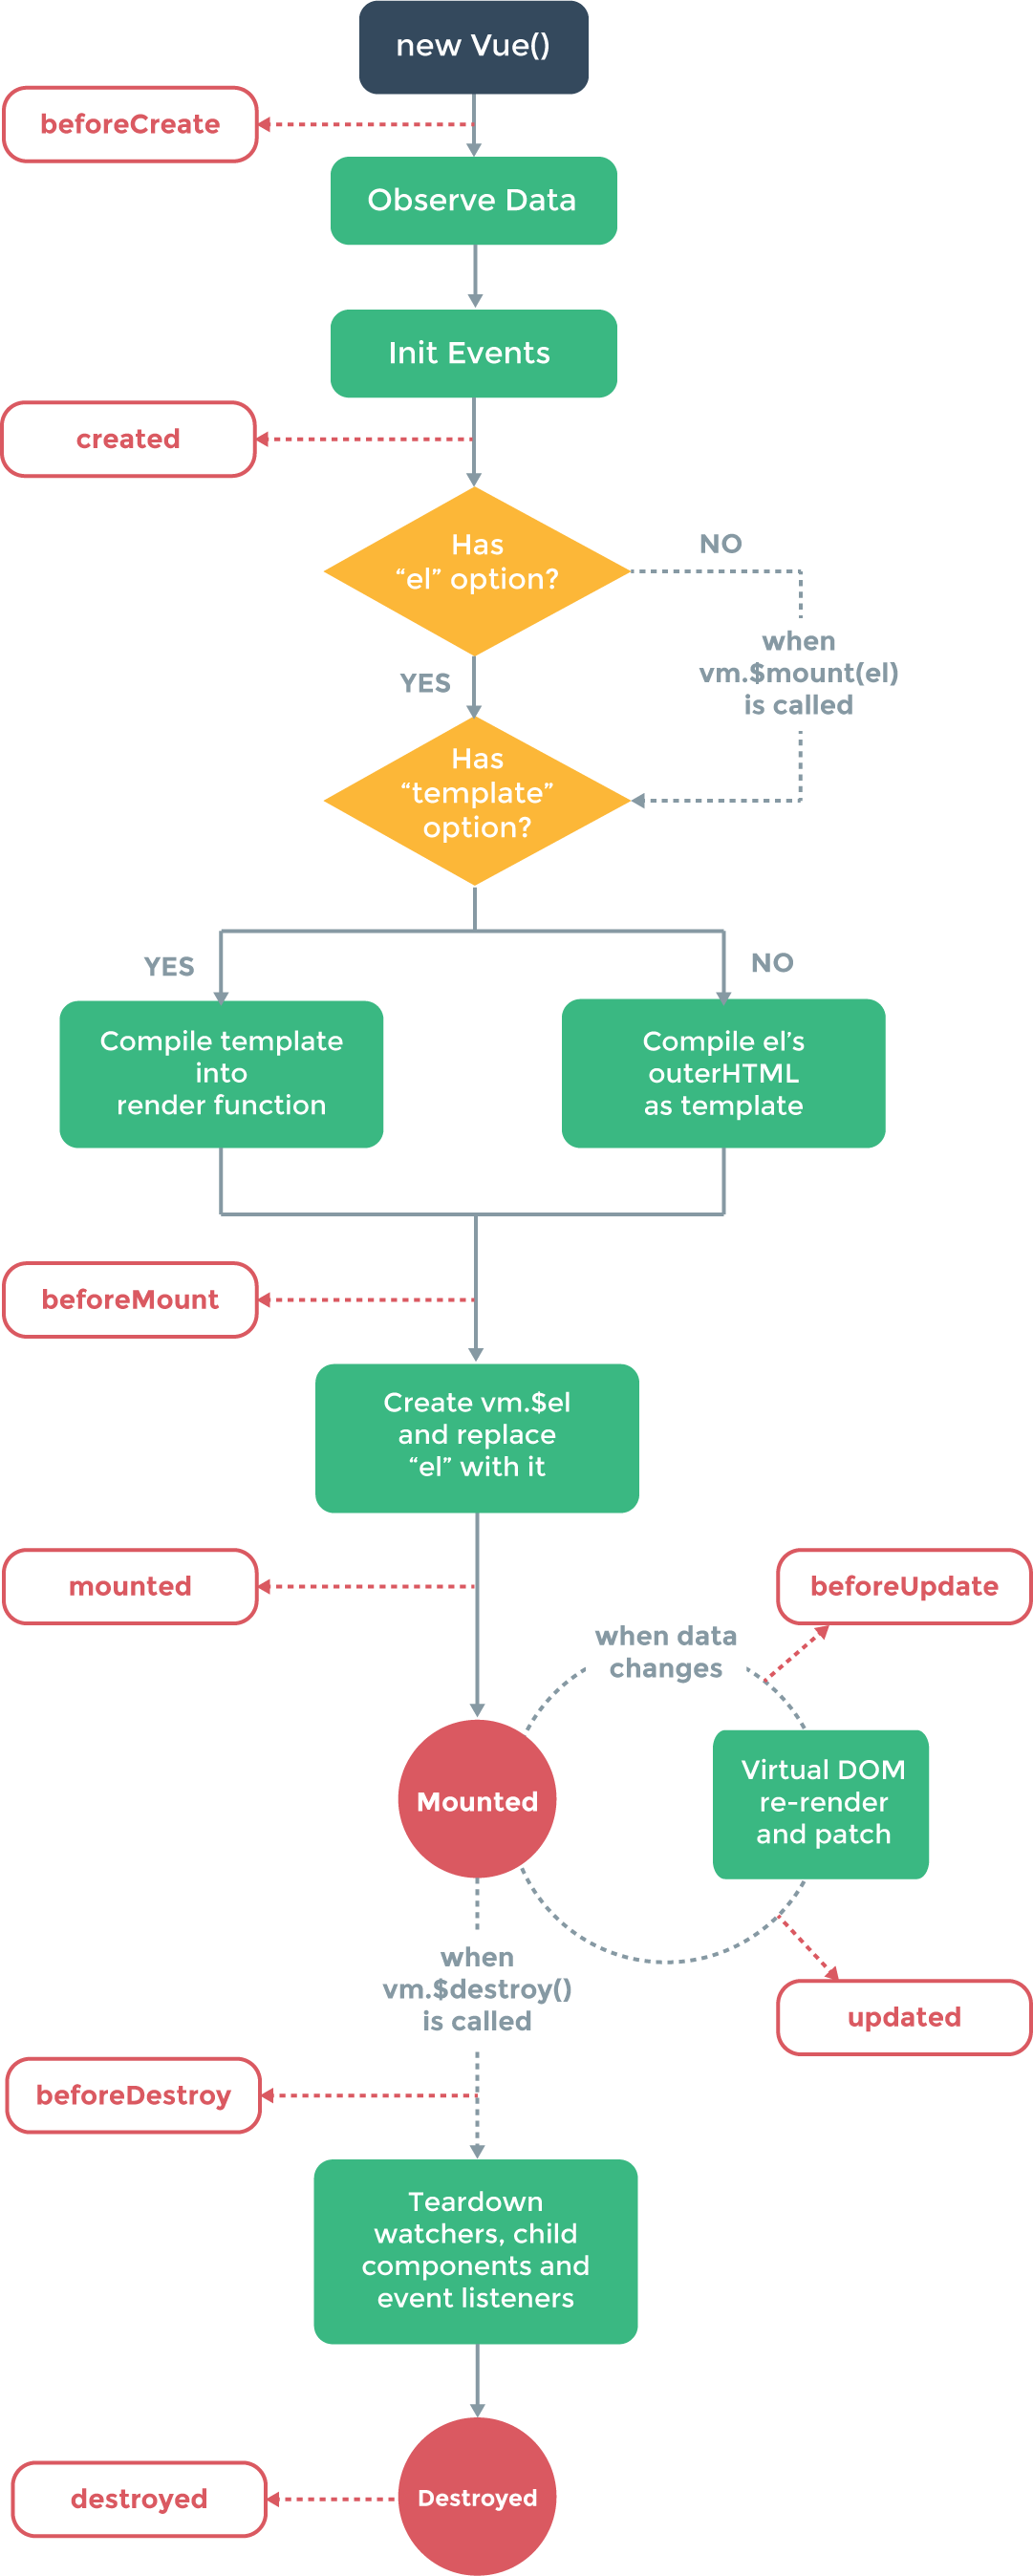
\includegraphics[scale=0.25]{lifecycle.png}
\caption{Vue实例的生命周期}
\end{figure}

每个 Vue 实例在被创建之前都要经过一系列的初始化过程。例如,实例需要配置数据观测(data observer)、编译模版、挂载实例到 DOM ,然后在数据变化时更新 DOM 。


\subsection{beforeCreate}


\subsection{created}


在Vue实例被创建的过程中,实例也会调用一些 生命周期钩子 ,这就给我们提供了执行自定义逻辑的机会。例如,created 这个钩子在实例被创建之后被调用:

\begin{lstlisting}[language=JavaScript]
var vm = new Vue({
  data: {
    a: 1
  },
  created: function () {
    // `this` 指向 vm 实例
    console.log('a is: ' + this.a)
  }
})
// -> "a is: 1"
\end{lstlisting}


\subsection{beforeUpdate}


\subsection{updated}




\subsection{beforeMount}



\subsection{mounted}


也有一些其它的钩子,在实例生命周期的不同阶段调用,如 mounted、 updated 、destroyed 。钩子的 this 指向调用它的 Vue 实例。

\subsection{beforeDestroy}


\subsection{destroyed}



Vue.js没有“控制器”的概念,组件的自定义逻辑可以分布在这些钩子中。

\chapter{Vue Template}


Vue.js 使用了基于 HTML 的模版语法,允许开发者声明式地将 DOM 绑定至底层 Vue 实例的数据。所有 Vue.js 的模板都是合法的 HTML ,所以能被遵循规范的浏览器和 HTML 解析器解析。


在底层的实现上, Vue 将模板编译成虚拟 DOM 渲染函数。结合响应系统,在应用状态改变时, Vue 能够智能地计算出重新渲染组件的最小代价并应用到 DOM 操作上。

如果熟悉虚拟 DOM,可以结合原生JavaScript代码,从而在不用模板,直接写渲染(render)函数,使用可选的 JSX 语法。

\section{Interpolation}


\subsection{Text}

数据绑定最常见的形式就是使用 “Mustache” 语法(双大括号)的文本插值:

\begin{lstlisting}[language=JavaScript]
<span>Message: {{ msg }}</span>
\end{lstlisting}

Mustache 标签将会被替代为对应数据对象上 msg 属性的值。无论何时,绑定的数据对象上 msg 属性发生了改变,插值处的内容都会更新。




通过使用 v-once 指令,你也能执行一次性地插值,当数据改变时,插值处的内容不会更新。但请留心这会影响到该节点上所有的数据绑定:

\begin{lstlisting}[language=JavaScript]
<span v-once>This will never change: {{ msg }}</span>
\end{lstlisting}




\subsection{HTML}

双大括号会将数据解释为纯文本,而非 HTML 。为了输出真正的 HTML ,你需要使用 v-html 指令:

\begin{lstlisting}[language=JavaScript]
<div v-html="rawHtml"></div>
\end{lstlisting}

被插入的内容都会被当做 HTML —— 数据绑定会被忽略。注意,你不能使用 v-html 来复合局部模板,因为 Vue 不是基于字符串的模板引擎。组件更适合担任 UI 重用与复合的基本单元。

站点上动态渲染的任意 HTML 可能会非常危险,因为它很容易导致 XSS 攻击。请只对可信内容使用 HTML 插值,绝不要对用户提供的内容插值。




\subsection{Attribute}

Mustache 不能在 HTML 属性中使用,应使用 v-bind 指令:

\begin{lstlisting}[language=JavaScript]
<div v-bind:id="dynamicId"></div>
\end{lstlisting}

这对布尔值的属性也有效 —— 如果条件被求值为 false 的话该属性会被移除:

\begin{lstlisting}[language=JavaScript]
<button v-bind:disabled="someDynamicCondition">Button</button>
\end{lstlisting}





\subsection{Expression}

在模板中除了绑定简单的属性键值之外,对于所有的数据绑定, Vue.js 都提供了完全的 JavaScript 表达式支持。

\begin{lstlisting}[language=JavaScript]
{{ number + 1 }}
{{ ok ? 'YES' : 'NO' }}
{{ message.split('').reverse().join('') }}
<div v-bind:id="'list-' + id"></div>
\end{lstlisting}


这些表达式会在所属 Vue 实例的数据作用域下作为 JavaScript 被解析。有个限制就是,每个绑定都只能包含单个表达式,所以下面的例子都不会生效。

\begin{lstlisting}[language=JavaScript]
<!-- 这是语句,不是表达式 -->
{{ var a = 1 }}
<!-- 流控制也不会生效,请使用三元表达式 -->
{{ if (ok) { return message } }}
\end{lstlisting}


模板表达式都被放在沙盒中,只能访问全局变量的一个白名单,如 Math 和 Date 。你不应该在模板表达式中试图访问用户定义的全局变量。




\section{Directive}

指令(Directives)是带有 v- 前缀的特殊属性。指令属性的值预期是单一 JavaScript 表达式(除了 v-for,之后再讨论)。指令的职责就是当其表达式的值改变时相应地将某些行为应用到 DOM 上。

\begin{lstlisting}[language=JavaScript]
<p v-if="seen">Now you see me</p>
\end{lstlisting}

这里, v-if 指令将根据表达式 seen 的值的真假来移除/插入 <p> 元素。


\begin{lstlisting}[language=JavaScript]

\end{lstlisting}




\subsection{Argument}

一些指令能接受一个“参数”,在指令后以冒号指明。例如, v-bind 指令被用来响应地更新 HTML 属性:

\begin{lstlisting}[language=JavaScript]
<a v-bind:href="url"></a>
\end{lstlisting}

在这里 href 是参数,告知 v-bind 指令将该元素的 href 属性与表达式 url 的值绑定。

另一个例子是 v-on 指令,它用于监听 DOM 事件:

\begin{lstlisting}[language=JavaScript]
<a v-on:click="doSomething">
\end{lstlisting}

在这里参数是监听的事件名。

\subsection{Modifier}

修饰符(Modifiers)是以半角句号 . 指明的特殊后缀,用于指出一个指定应该以特殊方式绑定。例如,.prevent 修饰符告诉 v-on 指令对于触发的事件调用 event.preventDefault():

\begin{lstlisting}[language=JavaScript]
<form v-on:submit.prevent="onSubmit"></form>
\end{lstlisting}


\section{Filter}

Vue.js allows you to define filters that can be used to apply common text formatting. Filters are usable in two places: mustache interpolations and v-bind expressions. Filters should be appended to the end of the JavaScript expression, denoted by the “pipe” symbol:

Vue.js 允许自定义过滤器,被用作一些常见的文本格式化。过滤器应该被添加在 mustache 插值的尾部,由“管道符”指示:


\begin{lstlisting}[language=JavaScript]
{{ message | capitalize }}
\end{lstlisting}




\begin{lstlisting}[language=JavaScript]
<!-- in mustaches -->
{{ message | capitalize }}
<!-- in v-bind -->
<div v-bind:id="rawId | formatId"></div>
\end{lstlisting}


Vue 2.x 中,过滤器只能在 mustache 绑定和 v-bind 表达式(从 2.1.0 开始支持)中使用,因为过滤器设计目的就是用于文本转换。为了在其他指令中实现更复杂的数据变换,你应该使用计算属性。

过滤器函数总接受表达式的值作为第一个参数。



\begin{lstlisting}[language=JavaScript]
new Vue({
  // ...
  filters: {
    capitalize: function (value) {
      if (!value) return ''
      value = value.toString()
      return value.charAt(0).toUpperCase() + value.slice(1)
    }
  }
})
\end{lstlisting}



过滤器可以串联:

\begin{lstlisting}[language=JavaScript]
{{ message | filterA | filterB }}
\end{lstlisting}

过滤器本身是 JavaScript 函数,因此可以接受参数:

\begin{lstlisting}[language=JavaScript]
{{ message | filterA('arg1', arg2) }}
\end{lstlisting}

这里,字符串 \texttt{'arg1'} 将传给过滤器作为第二个参数, arg2 表达式的值将被求值然后传给过滤器作为第三个参数。



\section{Shorthand}


v- 前缀在模板中是作为一个标示 Vue 特殊属性的明显标识。

当使用 Vue.js 为现有的标记添加动态行为时,它会很有用,但对于一些经常使用的指令来说有点繁琐。同时,当搭建 Vue.js 管理所有模板的 SPA 时,v- 前缀也变得没那么重要了,因此Vue.js 为两个最为常用的指令v-bind和v-on提供了特别的缩写。

虽然它们看起来可能与普通的 HTML 略有不同,但是\texttt{:}与\texttt{@}对于属性名来说都是合法字符,在所有支持 Vue.js 的浏览器都能被正确地解析,而且它们不会出现在最终渲染的标记,缩写语法是完全可选的。


\subsection{v-bind}




\begin{lstlisting}[language=JavaScript]
<!-- 完整语法 -->
<a v-bind:href="url"></a>
<!-- 缩写 -->
<a :href="url"></a>
\end{lstlisting}


\subsection{v-on}



\begin{lstlisting}[language=JavaScript]
<!-- 完整语法 -->
<a v-on:click="doSomething"></a>
<!-- 缩写 -->
<a @click="doSomething"></a>
\end{lstlisting}

\chapter{Vue Property}


\section{Computed Property}


在模板中绑定表达式是非常便利的,但是它们实际上只用于简单的操作。在模板中放入太多的逻辑会让模板过重且难以维护。例如:

\begin{lstlisting}[language=JavaScript]
<div id="example">
  {{ message.split('').reverse().join('') }}
</div>
\end{lstlisting}

在实现反向显示 message 之前都应该确认它,这个问题在需要不止一次反向显示 message 的时候变得更加糟糕,因此任何复杂逻辑都应当使用计算属性。



\begin{lstlisting}[language=JavaScript]
<div id="example">
  <p>Original message: "{{ message }}"</p>
  <p>Computed reversed message: "{{ reversedMessage }}"</p>
</div>

<script>
var vm = new Vue({
  el: '#example',
  data: {
    message: 'Hello'
  },
  computed: {
    // a computed getter
    reversedMessage: function () {
      // `this` points to the vm instance
      return this.message.split('').reverse().join('')
    }
  }
})
</script>
\end{lstlisting}

结果如下:


\begin{lstlisting}[language=JavaScript]
Original message: "Hello"
Computed reversed message: "olleH"
\end{lstlisting}

这里我们声明了一个计算属性 reversedMessage,其提供的函数将用作属性 vm.reversedMessage 的 getter 。


\begin{lstlisting}[language=JavaScript]
console.log(vm.reversedMessage) // -> 'olleH'
vm.message = 'Goodbye'
console.log(vm.reversedMessage) // -> 'eybdooG'
\end{lstlisting}

在浏览器的控制台中修改 vm,\texttt{vm.reversedMessage}的值始终取决于 vm.message 的值。


可以像绑定普通属性一样在模板中绑定计算属性。 Vue 知道 vm.reversedMessage 依赖于 vm.message ,因此当 vm.message 发生改变时,依赖于 vm.reversedMessage 的绑定也会更新。而且最妙的是我们是声明式地创建这种依赖关系:计算属性的 getter 是干净无副作用的,因此也是易于测试和理解的。


\section{Computed Cache}

可以通过调用表达式中的method来达到和上述同样的效果:


\begin{lstlisting}[language=JavaScript]
<p>Reversed message: "{{ reverseMessage() }}"</p>

<script>
// in component
methods: {
  reverseMessage: function () {
    return this.message.split('').reverse().join('')
  }
}
</script>
\end{lstlisting}

不经过计算属性,我们可以在 method 中定义一个相同的函数来替代它。对于最终的结果,两种方式确实是相同的。然而,不同的是计算属性是基于它的依赖缓存。计算属性只有在它的相关依赖发生改变时才会重新取值。这就意味着只要 message 没有发生改变,多次访问 reversedMessage 计算属性会立即返回之前的计算结果,而不必再次执行函数。

这也同样意味着如下计算属性将不会更新,因为 Date.now() 不是响应式依赖:

\begin{lstlisting}[language=JavaScript]
computed: {
  now: function () {
    return Date.now()
  }
}
\end{lstlisting}

相比而言,每当重新渲染的时候,method 调用总会执行函数。

我们为什么需要缓存?假设我们有一个重要的计算属性 A ,这个计算属性需要一个巨大的数组遍历和做大量的计算。然后我们可能有其他的计算属性依赖于 A 。如果没有缓存,我们将不可避免的多次执行 A 的 getter !如果你不希望有缓存,请用 method 替代。

\section{Watched Property}

Vue.js 提供了一个方法 \$watch ,它用于观察 Vue 实例上的数据变动。当一些数据需要根据其它数据变化时, \$watch 很诱人 —— 特别是如果你来自 AngularJS 。不过,通常更好的办法是使用计算属性而不是一个命令式的 \$watch 回调。

思考下面例子:

\begin{lstlisting}[language=JavaScript]
<div id="demo">{{ fullName }}</div>

<script>
var vm = new Vue({
  el: '#demo',
  data: {
    firstName: 'Foo',
    lastName: 'Bar',
    fullName: 'Foo Bar'
  },
  watch: {
    firstName: function (val) {
      this.fullName = val + ' ' + this.lastName
    },
    lastName: function (val) {
      this.fullName = this.firstName + ' ' + val
    }
  }
})
</script>
\end{lstlisting}

上面代码是命令式的和重复的。跟计算属性对比:

\begin{lstlisting}[language=JavaScript]
var vm = new Vue({
  el: '#demo',
  data: {
    firstName: 'Foo',
    lastName: 'Bar'
  },
  computed: {
    fullName: function () {
      return this.firstName + ' ' + this.lastName
    }
  }
})
\end{lstlisting}

\section{Computed Setter}

计算属性默认只有 getter ,不过在需要时你也可以提供一个 setter :


\begin{lstlisting}[language=JavaScript]
// ...
computed: {
  fullName: {
    // getter
    get: function () {
      return this.firstName + ' ' + this.lastName
    },
    // setter
    set: function (newValue) {
      var names = newValue.split(' ')
      this.firstName = names[0]
      this.lastName = names[names.length - 1]
    }
  }
}
// ...
\end{lstlisting}


在运行 vm.fullName = 'John Doe' 时, setter 会被调用, vm.firstName 和 vm.lastName 也会被对应更新。

\chapter{Vue Watcher}


虽然计算属性在大多数情况下更合适,但有时也需要一个自定义的 watcher 。这是为什么 Vue 提供一个更通用的方法通过 watch 选项,来响应数据的变化。当你想要在数据变化响应时,执行异步操作或开销较大的操作,这是很有用的。



\begin{lstlisting}[language=JavaScript]
<div id="watch-example">
  <p>
    Ask a yes/no question:
    <input v-model="question">
  </p>
  <p>{{ answer }}</p>
</div>
\end{lstlisting}



\begin{lstlisting}[language=JavaScript]
<!-- Since there is already a rich ecosystem of ajax libraries    -->
<!-- and collections of general-purpose utility methods, Vue core -->
<!-- is able to remain small by not reinventing them. This also   -->
<!-- gives you the freedom to just use what you're familiar with. -->
<script src="https://unpkg.com/axios@0.12.0/dist/axios.min.js"></script>
<script src="https://unpkg.com/lodash@4.13.1/lodash.min.js"></script>
<script>
var watchExampleVM = new Vue({
  el: '#watch-example',
  data: {
    question: '',
    answer: 'I cannot give you an answer until you ask a question!'
  },
  watch: {
    // 如果 question 发生改变,这个函数就会运行
    question: function (newQuestion) {
      this.answer = 'Waiting for you to stop typing...'
      this.getAnswer()
    }
  },
  methods: {
    // _.debounce 是一个通过 lodash 限制操作频率的函数。
    // 在这个例子中,我们希望限制访问yesno.wtf/api的频率
    // ajax请求直到用户输入完毕才会发出
    // 学习更多关于 _.debounce function (and its cousin
    // _.throttle), 参考: https://lodash.com/docs#debounce
    getAnswer: _.debounce(
      function () {
        var vm = this
        if (this.question.indexOf('?') === -1) {
          vm.answer = 'Questions usually contain a question mark. ;-)'
          return
        }
        vm.answer = 'Thinking...'
        axios.get('https://yesno.wtf/api')
          .then(function (response) {
            vm.answer = _.capitalize(response.data.answer)
          })
          .catch(function (error) {
            vm.answer = 'Error! Could not reach the API. ' + error
          })
      },
      // 这是我们为用户停止输入等待的毫秒数
      500
    )
  }
})
</script>
\end{lstlisting}

在这个示例中,使用 watch 选项允许我们执行异步操作(访问一个 API),限制我们执行该操作的频率,并在我们得到最终结果前,设置中间状态。这是计算属性无法做到的。

除了 watch 选项之外,还可以使用 vm.\$watch API 命令。


\chapter{Vue Binding}


数据绑定一个常见需求是操作元素的 class 列表和它的内联样式。因为它们都是属性 ,可以用v-bind 处理它们:只需要计算出表达式最终的字符串。不过,字符串拼接麻烦又易错,因此在 v-bind 用于 class 和 style 时, Vue.js 专门增强了它。



现在,表达式的结果类型除了字符串之外,还可以是对象或数组。


\section{Binding HTML Classes}



\subsection{Object Syntax}

可以传给\texttt{v-bind:class} 一个对象来动态地切换 class 。

\begin{lstlisting}[language=JavaScript]
<div v-bind:class="{ active: isActive }"></div>
\end{lstlisting}

上面的语法表示 class~active 的更新将取决于数据属性 isActive 是否为真值 。

也可以在对象中传入更多属性用来动态切换多个 class 。

此外, \texttt{v-bind:class}指令可以与普通的 class 属性共存。

\begin{compactitem}
\item 模板

\begin{lstlisting}[language=JavaScript]
<div class="static"
     v-bind:class="{ active: isActive, 'text-danger': hasError }">
</div>
\end{lstlisting}

\item 数据

\begin{lstlisting}[language=JavaScript]
data: {
  isActive: true,
  hasError: false
}
\end{lstlisting}
\end{compactitem}



最终被渲染为:


\begin{lstlisting}[language=JavaScript]
<div class="static active"></div>
\end{lstlisting}

当 isActive 或者 hasError 变化时,class 列表将相应地更新。例如,如果 hasError 的值为 true , class列表将变为\texttt{"static active text-danger"}。

也可以直接绑定数据里的一个对象:

\begin{lstlisting}[language=JavaScript]
<div v-bind:class="classObject"></div>
\end{lstlisting}

对应的数据为:

\begin{lstlisting}[language=JavaScript]
data: {
  classObject: {
    active: true,
    'text-danger': false
  }
}
\end{lstlisting}

最终的渲染的结果和上面一样,也可以在这里绑定返回对象的计算属性,这是一个常用且强大的模式:

\begin{lstlisting}[language=JavaScript]
<div v-bind:class="classObject"></div>

<script>
data: {
  isActive: true,
  error: null
},
computed: {
  classObject: function () {
    return {
      active: this.isActive && !this.error,
      'text-danger': this.error && this.error.type === 'fatal',
    }
  }
}
</script>
\end{lstlisting}


\subsection{Array Syntax}

可以把一个数组传给 \texttt{v-bind:class} 以应用一个 class 列表:


\begin{lstlisting}[language=JavaScript]
<div v-bind:class="[activeClass, errorClass]">
\end{lstlisting}

对应的数据:

\begin{lstlisting}[language=JavaScript]
data: {
  activeClass: 'active',
  errorClass: 'text-danger'
}
\end{lstlisting}

最终被渲染为:

\begin{lstlisting}[language=JavaScript]
<div class="active text-danger"></div>
\end{lstlisting}

如果需要根据条件切换列表中的 class ,可以用三元表达式:


\begin{lstlisting}[language=JavaScript]
<div v-bind:class="[isActive ? activeClass : '', errorClass]">
\end{lstlisting}

此例始终添加 errorClass ,但是只有在 isActive 是 true 时添加 activeClass 。

不过,当有多个条件 class 时这样写有些繁琐。可以在数组语法中使用对象语法:

\begin{lstlisting}[language=JavaScript]
<div v-bind:class="[{ active: isActive }, errorClass]">
\end{lstlisting}




\subsection{With Components}

在一个定制的组件上用到 class 属性的时候,这些类将被添加到根元素上面,这个元素上已经存在的类不会被覆盖。

例如,在声明一个组件my-component来使用class属性:

\begin{lstlisting}[language=JavaScript]
Vue.component('my-component',{
   template: '<p class="foo bar">Hi</p>'
})
\end{lstlisting}

在使用它的时候添加一些 class:

\begin{lstlisting}[language=JavaScript]
<my-component class="baz boo"></my-component>
\end{lstlisting}

HTML 最终将被渲染成为:


\begin{lstlisting}[language=JavaScript]
<p class="foo bar baz boo">Hi</p>
\end{lstlisting}

同样的适用于绑定 HTML class :

\begin{lstlisting}[language=JavaScript]
<my-component v-bind:class="{ active: isActive }"></my-component>
\end{lstlisting}

当 isActive 为 true 的时候,HTML 将被渲染成为:


\begin{lstlisting}[language=JavaScript]
<p class="foo bar active"></p>
\end{lstlisting}








\section{Binding Inline Styles}



\subsection{Object Syntax}

v-bind:style 的对象语法十分直观——看着非常像 CSS ,其实它是一个 JavaScript 对象。 CSS 属性名可以用驼峰式(camelCase)或短横分隔命名(kebab-case):


\begin{lstlisting}[language=JavaScript]
<div v-bind:style="{ color: activeColor, fontSize: fontSize + 'px' }"></div>

<script>
data: {
  activeColor: 'red',
  fontSize: 30
}
</script>
\end{lstlisting}

直接绑定到一个样式对象通常更好,让模板更清晰:


\begin{lstlisting}[language=JavaScript]
<div v-bind:style="styleObject"></div>

<script>
data: {
  styleObject: {
    color: 'red',
    fontSize: '13px'
  }
}
</script>
\end{lstlisting}

同样的,对象语法常常结合返回对象的计算属性使用。

\begin{lstlisting}[language=JavaScript]

\end{lstlisting}



\subsection{Array Syntax}

v-bind:style 的数组语法可以将多个样式对象应用到一个元素上:


\begin{lstlisting}[language=JavaScript]
<div v-bind:style="[baseStyles, overridingStyles]">
\end{lstlisting}



\begin{lstlisting}[language=JavaScript]

\end{lstlisting}



\begin{lstlisting}[language=JavaScript]

\end{lstlisting}


\subsection{Auto Prefixing}

当 v-bind:style 使用需要特定前缀的 CSS 属性时,如 transform ,Vue.js 会自动侦测并添加相应的前缀。




\chapter{Vue Component}

Vue的组件系统(Component)是 Vue.js 最强大的功能之一。


Vue组件可以扩展 HTML 元素,封装可重用的代码。

\begin{compactitem}
\item 在较高层面上,组件是自定义元素, Vue.js 的编译器为它添加特殊功能。
\item 在有些情况下,组件也可以是原生 HTML 元素的形式,以 is 特性扩展。
\end{compactitem}


注册一个Vue全局组件语法格式如下:




\begin{lstlisting}[language=JavaScript]
Vue.component(tagName,options)
\end{lstlisting}

其中,tagName为组件名,options为配置选项,在注册了一个Vue全局组件之后就可以使用如下的方式来调用:


\begin{lstlisting}[language=JavaScript]
<tagName></tagName>
\end{lstlisting}

对于自定义标签名tagName,Vue.js 不强制要求遵循 W3C规则 (小写并且包含一个短杠)。

\section{Register Component}


\subsection{Global Component}


默认情况下,Vue组件可以通过以下方式创建 :


\begin{lstlisting}[language=JavaScript]
new Vue({
  el: '#some-element',
  // 选项
})
\end{lstlisting}

要注册一个全局组件,可以使用 \texttt{Vue.component(tagName, options)},例如:

\begin{lstlisting}[language=JavaScript]
Vue.component('my-component', {
  // 选项
})
\end{lstlisting}


所有的Vue实例都可以使用全局组件。


\begin{lstlisting}[language=JavaScript]
<div id="app">
    <runoob></runoob>
</div>
 
<script>
// 注册全局组件
Vue.component('runoob', {
  template: '<h1>自定义组件!</h1>'
})
// 创建根实例
new Vue({
  el: '#app'
})
</script>
\end{lstlisting}

\begin{compactenum}
\item 注册全局组件(例如runoob)
\item 创建Vue实例(例如app)
\end{compactenum}


\begin{lstlisting}[language=JavaScript]

\end{lstlisting}





\subsection{Partial Component}

除了在全局注册每个组件,也可以在组件实例选项中注册局部组件,局部组件仅在实例/组件的内部作用域中可用:


\begin{lstlisting}[language=JavaScript]
var Child = {
  template: '<div>A custom component!</div>'
}
new Vue({
  // ...
  components: {
    // <my-component> 将只在父模板可用
    'my-component': Child
  }
})
\end{lstlisting}

这种封装也适用于其它可注册的 Vue 功能(如指令)。

\begin{lstlisting}[language=JavaScript]
<div id="app">
    <runoob></runoob>
</div>
 
<script>
var Child = {
  template: '<h1>自定义组件!</h1>'
}
 
// 创建根实例
new Vue({
  el: '#app',
  components: {
    // <runoob> 将只在父模板可用
    'runoob': Child
  }
})
</script>
\end{lstlisting}

\section{Custom Component}


Vue组件在注册之后,便可以在父实例的模块中以自定义元素 <my-component></my-component> 的形式使用,只要确保在初始化根实例 之前 注册了组件:


\begin{lstlisting}[language=JavaScript]
<div id="example">
  <my-component></my-component>
</div>

<script>
// 注册组件
Vue.component('my-component', {
  template: '<div>A custom component!</div>'
})
// 创建根实例
new Vue({
  el: '#example'
})
</script>
\end{lstlisting}

最终渲染为:

\begin{lstlisting}[language=JavaScript]
<div id="example">
  <div>A custom component!</div>
</div>
\end{lstlisting}




\begin{lstlisting}[language=JavaScript]

\end{lstlisting}




\begin{lstlisting}[language=JavaScript]

\end{lstlisting}



\section{Component Template}


当使用 DOM 作为组件的模版时(例如将 el 选项挂载到一个已存在的元素上), Vue会受到 HTML 的一些限制,因为 Vue 只有在浏览器解析和标准化 HTML 后才能获取模版内容。

尤其像 <ul>、 <ol>、<table>和<select>等元素限制了能被它包裹的元素, <option> 只能出现在其它元素内部。


在自定义组件中使用上述这些受限制的元素时会导致一些问题,例如:

\begin{lstlisting}[language=JavaScript]
<table>
  <my-row>...</my-row>
</table>
\end{lstlisting}

自定义组件 <my-row> 将会被认为是无效的内容,因此在渲染的时候会导致错误,Vue.js提供的变通的方案是使用特殊的 is 属性:

\begin{lstlisting}[language=JavaScript]
<table>
  <tr is="my-row"></tr>
</table>
\end{lstlisting}

注意,如果使用来自以下来源之一的字符串模板,这些限制将不适用,因此有必要的话推荐使用字符串模版。

\begin{compactitem}
\item \texttt{<script type="text/x-template">}
\item JavaScript内联模版字符串
\item .vue 组件
\end{compactitem}

HTML 特性不区分大小写。当使用非字符串模版时,prop的名字形式会从 camelCase 转为 kebab-case(短横线隔开):



\begin{lstlisting}[language=JavaScript]
Vue.component('child', {
  // camelCase in JavaScript
  props: ['myMessage'],
  template: '<span>{{ myMessage }}</span>'
})
\end{lstlisting}



\begin{lstlisting}[language=JavaScript]
<!-- kebab-case in HTML -->
<child my-message="hello!"></child>
\end{lstlisting}

实际上,如果使用字符串模版,不用在意这些限制。

\begin{lstlisting}[language=JavaScript]

\end{lstlisting}






\section{Component Composing}

组件意味着协同工作,通常父子组件会是这样的关系:组件 A 在它的模版中使用了组件 B ,它们之间必然需要相互通信——父组件要给子组件传递数据,子组件需要将它内部发生的事情告知给父组件。

在一个良好定义的接口中尽可能将父子组件解耦是很重要的,这样保证了每个组件可以在相对隔离的环境中书写和理解,也大幅提高了组件的可维护性和可重用性。



\begin{lstlisting}[language=JavaScript]

\end{lstlisting}




\begin{lstlisting}[language=JavaScript]

\end{lstlisting}




\begin{lstlisting}[language=JavaScript]

\end{lstlisting}





\begin{lstlisting}[language=JavaScript]

\end{lstlisting}



\begin{lstlisting}[language=JavaScript]

\end{lstlisting}





\begin{lstlisting}[language=JavaScript]

\end{lstlisting}



\begin{lstlisting}[language=JavaScript]

\end{lstlisting}



\begin{lstlisting}[language=JavaScript]

\end{lstlisting}




\begin{lstlisting}[language=JavaScript]

\end{lstlisting}



\begin{lstlisting}[language=JavaScript]

\end{lstlisting}



\begin{lstlisting}[language=JavaScript]

\end{lstlisting}




\chapter{Vue Event Handler}

Vue的事件监听的方式违背了关注点分离(separation of concern)传统理念。不必担心,因为所有的 Vue.js 事件处理方法和表达式都严格绑定在当前视图的 ViewModel 上,它不会导致任何维护上的困难。实际上,使用 v-on 有几个好处:

\begin{compactitem}
\item 在HTML模板中可以轻松定位在 JavaScript 代码里对应的方法。

\item 无须在 JavaScript 里手动绑定事件,ViewModel 代码可以是非常纯粹的逻辑,和 DOM 完全解耦,更易于测试。
\item 当一个 ViewModel 被销毁时,所有的事件处理器都会自动被删除,无须担心如何自己清理它们。
\end{compactitem}

可以用 v-on 指令监听 DOM 事件来触发一些 JavaScript 代码。


\begin{lstlisting}[language=JavaScript]
<div id="example-1">
  <button v-on:click="counter += 1">增加 1</button>
  <p>这个按钮被点击了 {{ counter }} 次。</p>
</div>

<script>
var example1=new Vue({
  el: '#example-1',
  data: {
     counter: 0
  }
})
</script>
\end{lstlisting}



\begin{lstlisting}[language=JavaScript]

\end{lstlisting}



\begin{lstlisting}[language=JavaScript]

\end{lstlisting}

\section{Event Handler}

许多事件处理的逻辑都很复杂,所以直接把 JavaScript 代码写在 v-on 指令中是不可行的,因此 v-on 可以接收一个定义的方法来调用。

\begin{lstlisting}[language=JavaScript]
<div id="example-2">
  <!-- `greet` 是在下面定义的方法名 -->
  <button v-on:click="greet">Greet</button>
</div>

<script>
var example2 = new Vue({
  el: '#example-2',
  data: {
    name: 'Vue.js'
  },
  // 在 `methods` 对象中定义方法
  methods: {
    greet: function (event) {
      // `this` 在方法里指当前 Vue 实例
      alert('Hello ' + this.name + '!')
      // `event` 是原生 DOM 事件
      alert(event.target.tagName)
    }
  }
})
// 也可以用 JavaScript 直接调用方法
example2.greet() // -> 'Hello Vue.js!'
</script>
\end{lstlisting}



\begin{lstlisting}[language=JavaScript]

\end{lstlisting}



\begin{lstlisting}[language=JavaScript]

\end{lstlisting}


\section{Inline Handler}

除了直接绑定到一个方法,也可以用内联 JavaScript 语句:

\begin{lstlisting}[language=JavaScript]
<div id="example-3">
  <button v-on:click="say('hi')">Say hi</button>
  <button v-on:click="say('what')">Say what</button>
</div>

<script>
new Vue({
  el: '#example-3',
  methods: {
    say: function (message) {
      alert(message)
    }
  }
})
</script>
\end{lstlisting}

有时也需要在内联语句处理器中访问原生 DOM 事件,可以用特殊变量 \$event 把它传入方法:

\begin{lstlisting}[language=JavaScript]
<button v-on:click="warn('Form cannot be submitted yet.', $event)">Submit</button>

<script>
// ...
methods: {
  warn: function (message, event) {
    // 现在我们可以访问原生事件对象
    if (event) event.preventDefault()
    alert(message)
  }
}
</script>
\end{lstlisting}



\begin{lstlisting}[language=JavaScript]

\end{lstlisting}


\section{Event Modifier}


在事件处理程序中调用 event.preventDefault() 或 event.stopPropagation() 是非常常见的需求。尽管我们可以在 methods 中轻松实现这点,但更好的方式是:methods 只有纯粹的数据逻辑,而不是去处理 DOM 事件细节。

为了解决这个问题, Vue.js 为 v-on 提供了 事件修饰符。通过由点(.)表示的指令后缀来调用修饰符。

\subsection{.stop}

\begin{lstlisting}[language=JavaScript]
<!-- 阻止单击事件冒泡 -->
<a v-on:click.stop="doThis"></a>
\end{lstlisting}

\subsection{.prevent}

\begin{lstlisting}[language=JavaScript]
<!-- 提交事件不再重载页面 -->
<form v-on:submit.prevent="onSubmit"></form>
\end{lstlisting}


\begin{lstlisting}[language=JavaScript]
<!-- 修饰符可以串联  -->
<a v-on:click.stop.prevent="doThat"></a>
\end{lstlisting}

\begin{lstlisting}[language=JavaScript]
<!-- 只有修饰符 -->
<form v-on:submit.prevent></form>
\end{lstlisting}



\subsection{.capture}


\begin{lstlisting}[language=JavaScript]
<!-- 添加事件侦听器时使用事件捕获模式 -->
<div v-on:click.capture="doThis">...</div>
\end{lstlisting}

\subsection{.self}

\begin{lstlisting}[language=JavaScript]
<!-- 只当事件在该元素本身(而不是子元素)触发时触发回调 -->
<div v-on:click.self="doThat">...</div>
\end{lstlisting}

\subsection{.once}

\begin{lstlisting}[language=JavaScript]
<!-- the click event will be triggered at most once -->
<a v-on:click.once="doThis"></a>
\end{lstlisting}




Unlike the other modifiers, which are exclusive to native DOM events, the .once modifier can also be used on component events. If you haven’t read about components yet, don’t worry about this for now.








\section{Key Modifier}



在监听键盘事件时,我们经常需要监测常见的键值。 Vue 允许为 v-on 在监听键盘事件时添加按键修饰符:



\begin{lstlisting}[language=JavaScript]
<!-- 只有在 keyCode 是 13 时调用 vm.submit() -->
<input v-on:keyup.13="submit">
\end{lstlisting}

 Vue 为最常用的按键提供了别名:

\begin{lstlisting}[language=JavaScript]
<!-- 同上 -->
<input v-on:keyup.enter="submit">
<!-- 缩写语法 -->
<input @keyup.enter="submit">
\end{lstlisting}

全部的按键别名如下:

\begin{compactitem}
\item .enter
\item .tab
\item .delete (捕获 “删除” 和 “退格” 键)
\item .esc
\item .space
\item .up
\item .down
\item .left
\item .right
\end{compactitem}

可以通过全局 config.keyCodes 对象自定义按键修饰符别名:

\begin{lstlisting}[language=JavaScript]
// 可以使用 v-on:keyup.f1
Vue.config.keyCodes.f1 = 112
\end{lstlisting}







\section{Modifier Key}


可以用如下修饰符开启鼠标或键盘事件监听,使在按键按下时发生响应。


\begin{compactitem}
\item .ctrl
\item .alt
\item .shift
\item .meta
\end{compactitem}

On Macintosh keyboards, meta is the command key (⌘). On Windows keyboards, meta is the windows key (⊞). On Sun Microsystems keyboards, meta is marked as a solid diamond (◆). On certain keyboards, specifically MIT and Lisp machine keyboards and successors, such as the Knight keyboard, space-cadet keyboard, meta is labeled “META”. On Symbolics keyboards, meta is labeled “META” or “Meta”.

\begin{lstlisting}[language=JavaScript]
<!-- Alt + C -->
<input @keyup.alt.67="clear">
<!-- Ctrl + Click -->
<div @click.ctrl="doSomething">Do something</div>
\end{lstlisting}


\begin{lstlisting}[language=JavaScript]

\end{lstlisting}



\begin{lstlisting}[language=JavaScript]

\end{lstlisting}